\usepackage{pgf}
\usepackage{tikz}
\usetikzlibrary{arrows,automata,fit}
\usetikzlibrary{calc,positioning,shapes.geometric}
\usetikzlibrary{shapes}
\usetikzlibrary{er}

\newcommand { \key }[1]{ \underline {#1}}

\newcommand{\ejemplografo}{
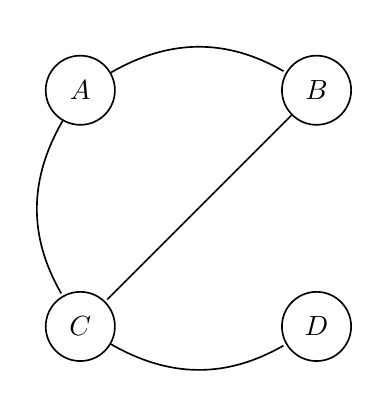
\begin{tikzpicture}[>=stealth',shorten >=1pt,auto,node distance=3cm,semithick]
  \tikzstyle{every state}=[draw=black,text=black]

  \node[state]         (A)                    {$A$};
  \node[state]         (B) [right of=A]       {$B$};
  \node[state]         (C) [below of=A]       {$C$};
  \node[state]         (D) [right of=C]       {$D$};
  
  \path (A) edge  [bend left]   node {}  (B)
            edge  [bend right]  node {}  (C)
        (B) edge                node {}  (C)
        (C) edge  [bend right]  node {}  (D);
\end{tikzpicture}}

\newcommand{\ejemplografocompleto}{
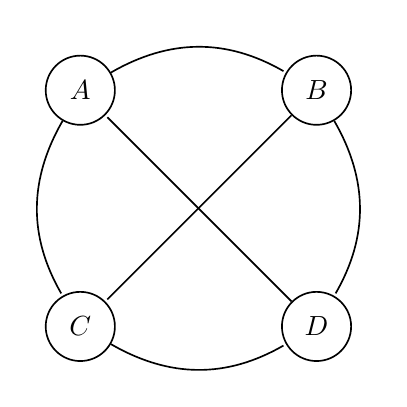
\begin{tikzpicture}[>=stealth',shorten >=1pt,auto,node distance=3cm,semithick]
  \tikzstyle{every state}=[draw=black,text=black]

  \node[state]         (A)                    {$A$};
  \node[state]         (B) [right of=A]       {$B$};
  \node[state]         (C) [below of=A]       {$C$};
  \node[state]         (D) [right of=C]       {$D$};
  
  \path (A) edge  [bend left]   node {}  (B)
            edge  [bend right]  node {}  (C)
		(B) edge  [bend left]   node {}  (D)
        (B) edge                node {}  (C)
        (D) edge                node {}  (A)
        (C) edge  [bend right]  node {}  (D);
\end{tikzpicture}}

\newcommand{\ejemplografodirigido}{
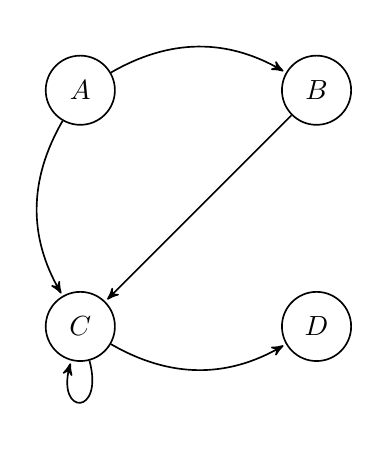
\begin{tikzpicture}[->,>=stealth',shorten >=1pt,auto,node distance=3cm,semithick]
  \tikzstyle{every state}=[draw=black,text=black]

  \node[state]         (A)                    {$A$};
  \node[state]         (B) [right of=A]       {$B$};
  \node[state]         (C) [below of=A]       {$C$};
  \node[state]         (D) [right of=C]       {$D$};
  
  \path (A) edge  [bend left]   node {}  (B)
            edge  [bend right]  node {}  (C)
        (B) edge                node {}  (C)
        (C) edge  [bend right]  node  {}  (D)
        (C) edge  [loop below]  node  {}  (C);
\end{tikzpicture}}

\newcommand{\ejemplosubgrafo}{
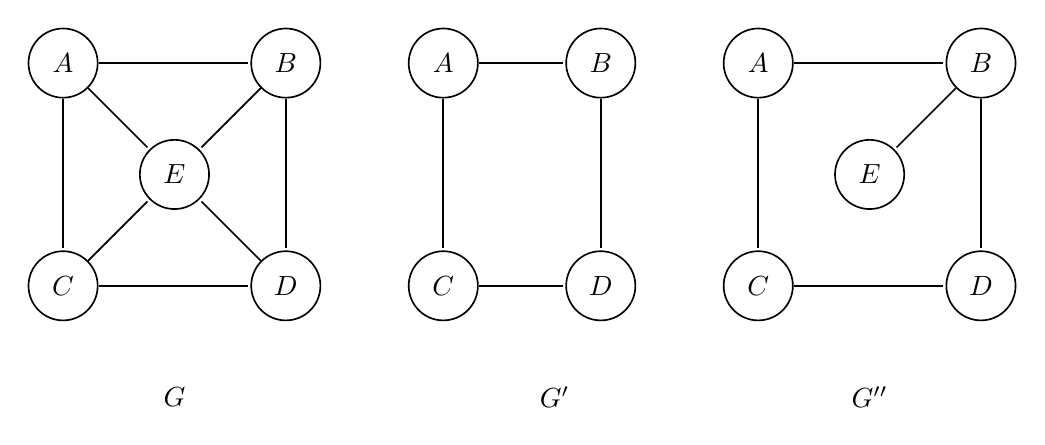
\begin{tikzpicture}[>=stealth',shorten >=1pt,auto,node distance=2cm,semithick]
  \tikzstyle{every state}=[draw=black,text=black]

% Grafo G
  \node[state]         (E)                          {$E$};
  \node[state]         (B) [above right of=E]       {$B$};
  \node[state]         (A) [above left of= E]       {$A$};
  \node[state]         (C) [below left of= E]       {$C$};
  \node[state]         (D) [below right of=E]       {$D$};

  \path (A) edge                node {}  (B)
        (A) edge                node {}  (E)
        (A) edge                node {}  (C)
        (B) edge                node {}  (D)
        (B) edge                node {}  (E)        
        (C) edge                node {}  (E)
        (C) edge                node {}  (D)
        (D) edge                node {}  (E);
        
        
% Subgrafo G'
  \node[state]         (F) [right of= B]       {$A$};
  \node[state]         (G) [right of= F]       {$B$};
  \node[state]         (H) [right of= D]       {$C$};
  \node[state]         (I) [right of= H]       {$D$};
  
  \path (F) edge                node {}  (G)
        (F) edge                node {}  (H)
        (G) edge                node {}  (I)
        (H) edge                node {}  (I);
        
% Subgrafo G'

  \node[state]         (J) [right of= G]             {$A$};
  \node[state]         (K) [right of= I]             {$C$};
  \node[state]         (N) [above right of= K]       {$E$};
  \node[state]         (M) [below right of= N]       {$D$};
  \node[state]         (L) [above right of= N]       {$B$};
  
  \path (J) edge                node {}  (K)
        (J) edge                node {}  (L)
        (L) edge                node {}  (N)
        (L) edge                node {}  (M)
        (K) edge                node {}  (M);
        
% Etiquetas con el nombre de los grafos
  \node[align=center, below right of=C] {$G$};
  \node[align=center, below right of=H] {$G'$};
  \node[align=center, below right of=K] {$G''$};
\end{tikzpicture}}

\newcommand{\ejemplounionintersecciongrafo}{
\begin{tikzpicture}[>=stealth',shorten >=1pt,auto,node distance=2cm,semithick]
  \tikzstyle{every state}=[draw=black,text=black]

% Grafo G
  \node[state]         (A)                          {$A$};
  \node[state]         (B) [below right of=A]       {$B$};
  \node[state]         (C) [below      of= B]       {$C$};
  \node[state]         (D) [right of=B]             {$D$};
  \node[state]         (E) [right of=C]             {$E$};

  \path (A) edge                node {}  (B)
        (B) edge                node {}  (C)
        (B) edge                node {}  (D)      
        (C) edge                node {}  (E)
        (D) edge                node {}  (E);
        
% Grafo G'
  \node[state]         (H) [right of= E]       {$C$};
  \node[state]         (I) [right of= D]       {$D$};
  \node[state]         (G) [right of= H]       {$E$};
  \node[state]         (F) [above right of= G] {$F$};
  
  \path (H) edge                node {}  (I)
        (I) edge                node {}  (F)
        (G) edge                node {}  (F)
        (H) edge                node {}  (G);
        
% Etiquetas con el nombre de los grafos
  \node[align=center, below right of=C] (Z) {$G$};
  \node[align=center, below right of=H] (Y) {$G'$};

% Grafo G \cup G'
  \node[state]         (J) [below left of=Z]        {$A$};
  \node[state]         (K) [below right of=J]       {$B$};
  \node[state]         (L) [below of= K]            {$C$};
  \node[state]         (M) [right of=K]             {$D$};
  \node[state]         (N) [right of=L]             {$E$};
  \node[state]         (R) [above right of=N]       {$F$};

  \path (J) edge                node {}  (K)
        (K) edge                node {}  (L)
        (K) edge                node {}  (M)      
        (L) edge                node {}  (N)
        (L) edge                node {}  (M)
        (N) edge                node {}  (R)
        (R) edge                node {}  (M)
        (M) edge                node {}  (N);
        
  \node[align=center, below right of=L] {$G \cup G'$};
  
% Grafo G \cup G'
  \node[state]         (O) [right of=R]        {$C$};
  \node[state]         (P) [right of=O]              {$E$};


  \path (O) edge                node {}  (P);
        
        
  \node[align=center, below right of=O] {$G \cap G'$};

\end{tikzpicture}}














\newcommand{\ejemplografoponderado}{
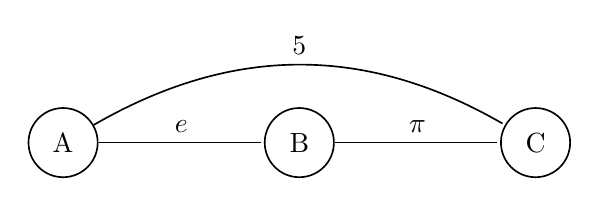
\begin{tikzpicture}[>=stealth',shorten >=1pt,auto,node distance=3cm,semithick]
  \tikzstyle{every state}=[draw=black,text=black]
 
  
  \node[state] (a)              {A};
  \node[state] (b) [right of=a] {B};
  \node[state] (c) [right of=b] {C};
  
  \path (a)     edge                node {$e$} (b);
  \path (a)   edge [bend left]   node {$5$} (c);  
  \path (b)   edge                node {$\pi$} (c);
 
  
\end{tikzpicture}}







\newcommand{\ejemplografocomplementario}{
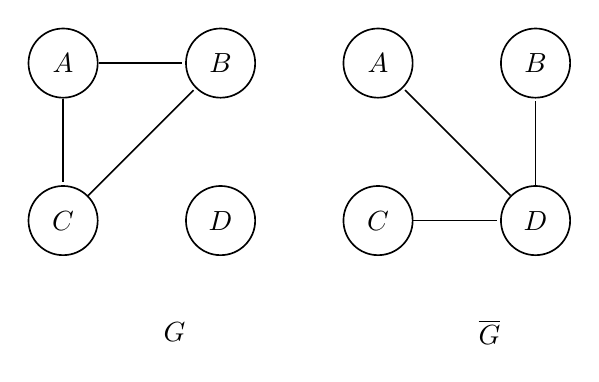
\begin{tikzpicture}[>=stealth',shorten >=1pt,auto,node distance=2cm,semithick]
  \tikzstyle{every state}=[draw=black,text=black]

% Grafo G
  \node[state]         (B)                          {$A$};
  \node[state]         (C) [below of=B]             {$C$};
  \node[state]         (D) [right of=B]             {$B$};
  \node[state]         (E) [right of=C]             {$D$};

  \path (B) edge                node {}  (C)
        (B) edge                node {}  (D)      
        (C) edge                node {}  (D);
        
% Grafo \overline{G}
  \node[state]         (H) [right of= E]       {$C$};
  \node[state]         (I) [right of= D]       {$A$};
  \node[state]         (G) [right of= H]       {$D$};
  \node[state]         (F) [right of= I]       {$B$};
  
  \path (G) edge                node {}  (I)
        (G) edge                node {}  (F)
        (H) edge                node {}  (G);
        
% Etiquetas con el nombre de los grafos
  \node[align=center, below right of=C] (Z) {$G$};
  \node[align=center, below right of=H] (Y) {$\overline{G}$};


\end{tikzpicture}}

\newcommand{\ejemplografodominancia}{
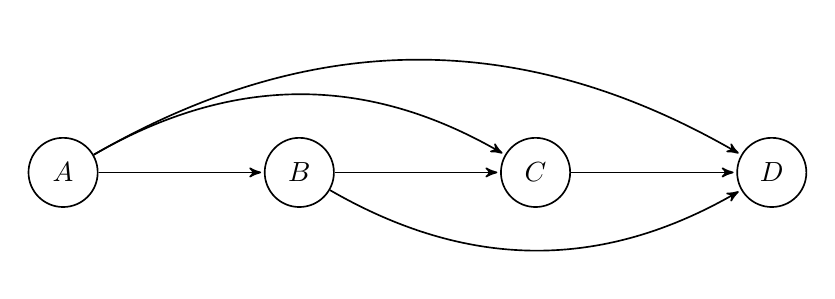
\begin{tikzpicture}[->,>=stealth',shorten >=1pt,auto,node distance=3cm,semithick]
  \tikzstyle{every state}=[draw=black,text=black]
 
  
  \node[state] (A)              {$A$};
  \node[state] (B) [right of=A] {$B$};
  \node[state] (C) [right of=B] {$C$};
  \node[state] (D) [right of=C] {$D$};
  
  \path (A) edge              node {} (B);
  \path (A) edge [bend left]  node {} (C);
  \path (A) edge [bend left]  node {} (D);
  \path (B) edge              node {} (C);
  \path (B) edge [bend right] node {} (D);
  \path (C) edge              node {} (D);
  
\end{tikzpicture}}

\newcommand{\ejemplografocompetitividad}{
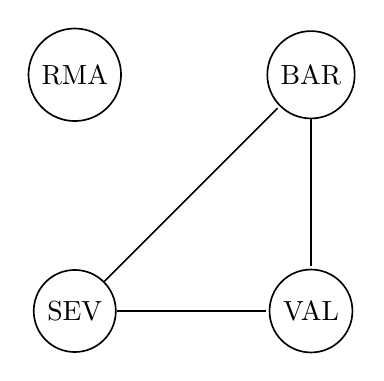
\begin{tikzpicture}[>=stealth',shorten >=1pt,auto,node distance=3cm,semithick]
  \tikzstyle{every state}=[draw=black,text=black]
 
  \node[state] (RMA)                      {RMA};
  \node[state] (BAR) [right       of=RMA] {BAR};
  \node[state] (SEV) [below       of=RMA] {SEV};
  \node[state] (VAL) [below       of=BAR] {VAL};
  
  \path (SEV)   edge                node {} (BAR);
  \path (SEV)   edge                node {} (VAL);  
  \path (BAR)   edge                node {} (VAL);
  
\end{tikzpicture}}

\newcommand{\ejemplografocompetitividadevolutivo}{
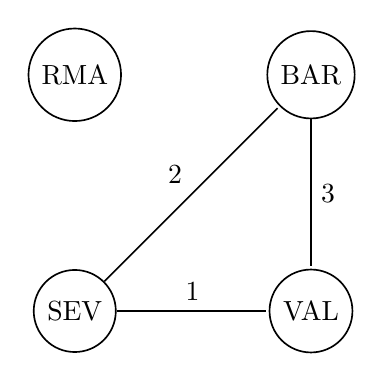
\begin{tikzpicture}[>=stealth',shorten >=1pt,auto,node distance=3cm,semithick]
  \tikzstyle{every state}=[draw=black,text=black]
 
  \node[state] (RMA)                      {RMA};
  \node[state] (BAR) [right       of=RMA] {BAR};
  \node[state] (SEV) [below       of=RMA] {SEV};
  \node[state] (VAL) [below       of=BAR] {VAL};
  
  \path (SEV)   edge                node {2} (BAR);
  \path (SEV)   edge                node {1} (VAL);  
  \path (BAR)   edge                node {3} (VAL);
  
\end{tikzpicture}}


\newcommand{\ejemplogradomedio}{
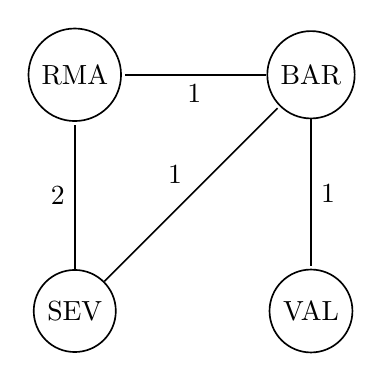
\begin{tikzpicture}[>=stealth',shorten >=1pt,auto,node distance=3cm,semithick]
  \tikzstyle{every state}=[draw=black,text=black]
 
  \node[state] (RMA)                      {RMA};
  \node[state] (BAR) [right       of=RMA] {BAR};
  \node[state] (SEV) [below       of=RMA] {SEV};
  \node[state] (VAL) [below       of=BAR] {VAL};
  
  \path (SEV)   edge                node {1} (BAR);
  \path (SEV)   edge                node {2} (RMA);  
  \path (BAR)   edge                node {1} (VAL);
  \path (BAR)   edge                node {1} (RMA);
  
\end{tikzpicture}}

\newcommand{\arquitectura}{
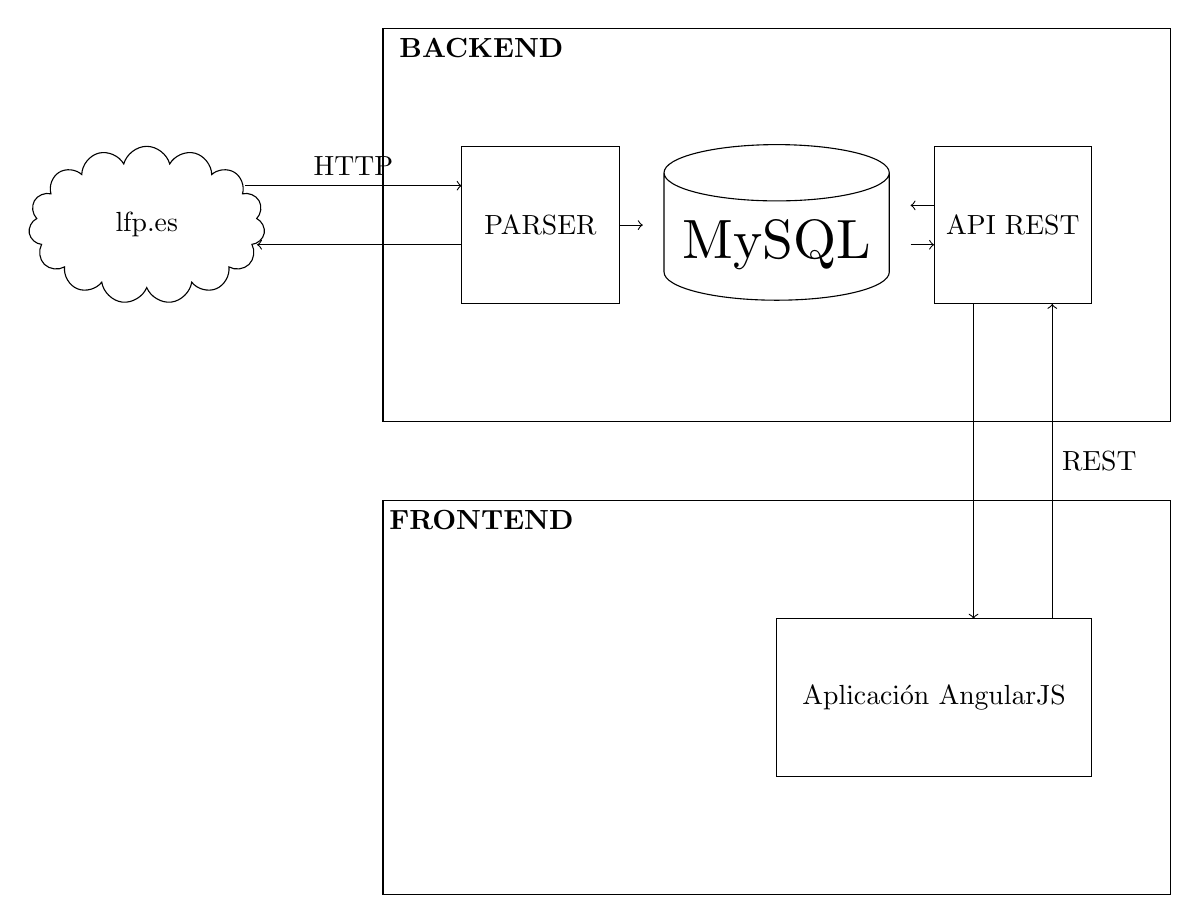
\begin{tikzpicture}[database/.style={
      cylinder,
      cylinder uses custom fill,
      cylinder body fill=white,
      cylinder end fill=white,
      shape border rotate=90,
      aspect=0.25,
      draw
    }]
 
 	% Base de datos
    \node[database, scale=2] at (5,2.25) (mysql) {MySQL};
    
    % Parser
    \draw (1,1.5) rectangle (3,3.5) node[midway] {PARSER};
       
    % API REST
    \draw (7,1.5) rectangle (9,3.5) node[midway] {API REST};
     
    % APP Angular
    \draw (5,-2.5) rectangle (9,-4.5) node[midway] {Aplicación AngularJS};
    
    % Nube
    \node[cloud, cloud puffs=15, cloud ignores aspect, minimum width=3cm, minimum height=2cm, align=center, draw] (cloud) at (-3, 2.5) {lfp.es};
     
    % Backend
    \draw (0,0) rectangle (10,5);
     
    % Frontend
    \draw (0,-6) rectangle (10,-1);
    
    % Flechas
    
    % Nube - Parser 
    \draw [->] (1, 2.25) -- node {}                  (-1.6, 2.25);
    \draw [<-] (1, 3) -- node[anchor=south] {HTTP}    (-1.75, 3);
    
    % Parser - MySQL
    \draw [->] (3, 2.50)   -- node {}  (3.3,2.50);
    
    % API REST - MySQL
    \draw [->] (6.7, 2.25)   -- node {}  (7.00,2.25);
    \draw [<-] (6.7, 2.75)   -- node {}  (7.00,2.75);
    
    % API REST - AngularJS
    \draw [->] (7.5, 1.5)   -- node {}      (7.5,-2.5);
    \draw [<-] (8.5, 1.5)   -- node[anchor=west] {REST}  (8.5,-2.5);
     
   	% Backend
 	\node at (1.25,4.75) {\textbf{BACKEND}};
 	
	% Frontend
 	\node at (1.25,-1.25) {\textbf{FRONTEND}};
 
\end{tikzpicture}}

\newcommand{\erparser}{
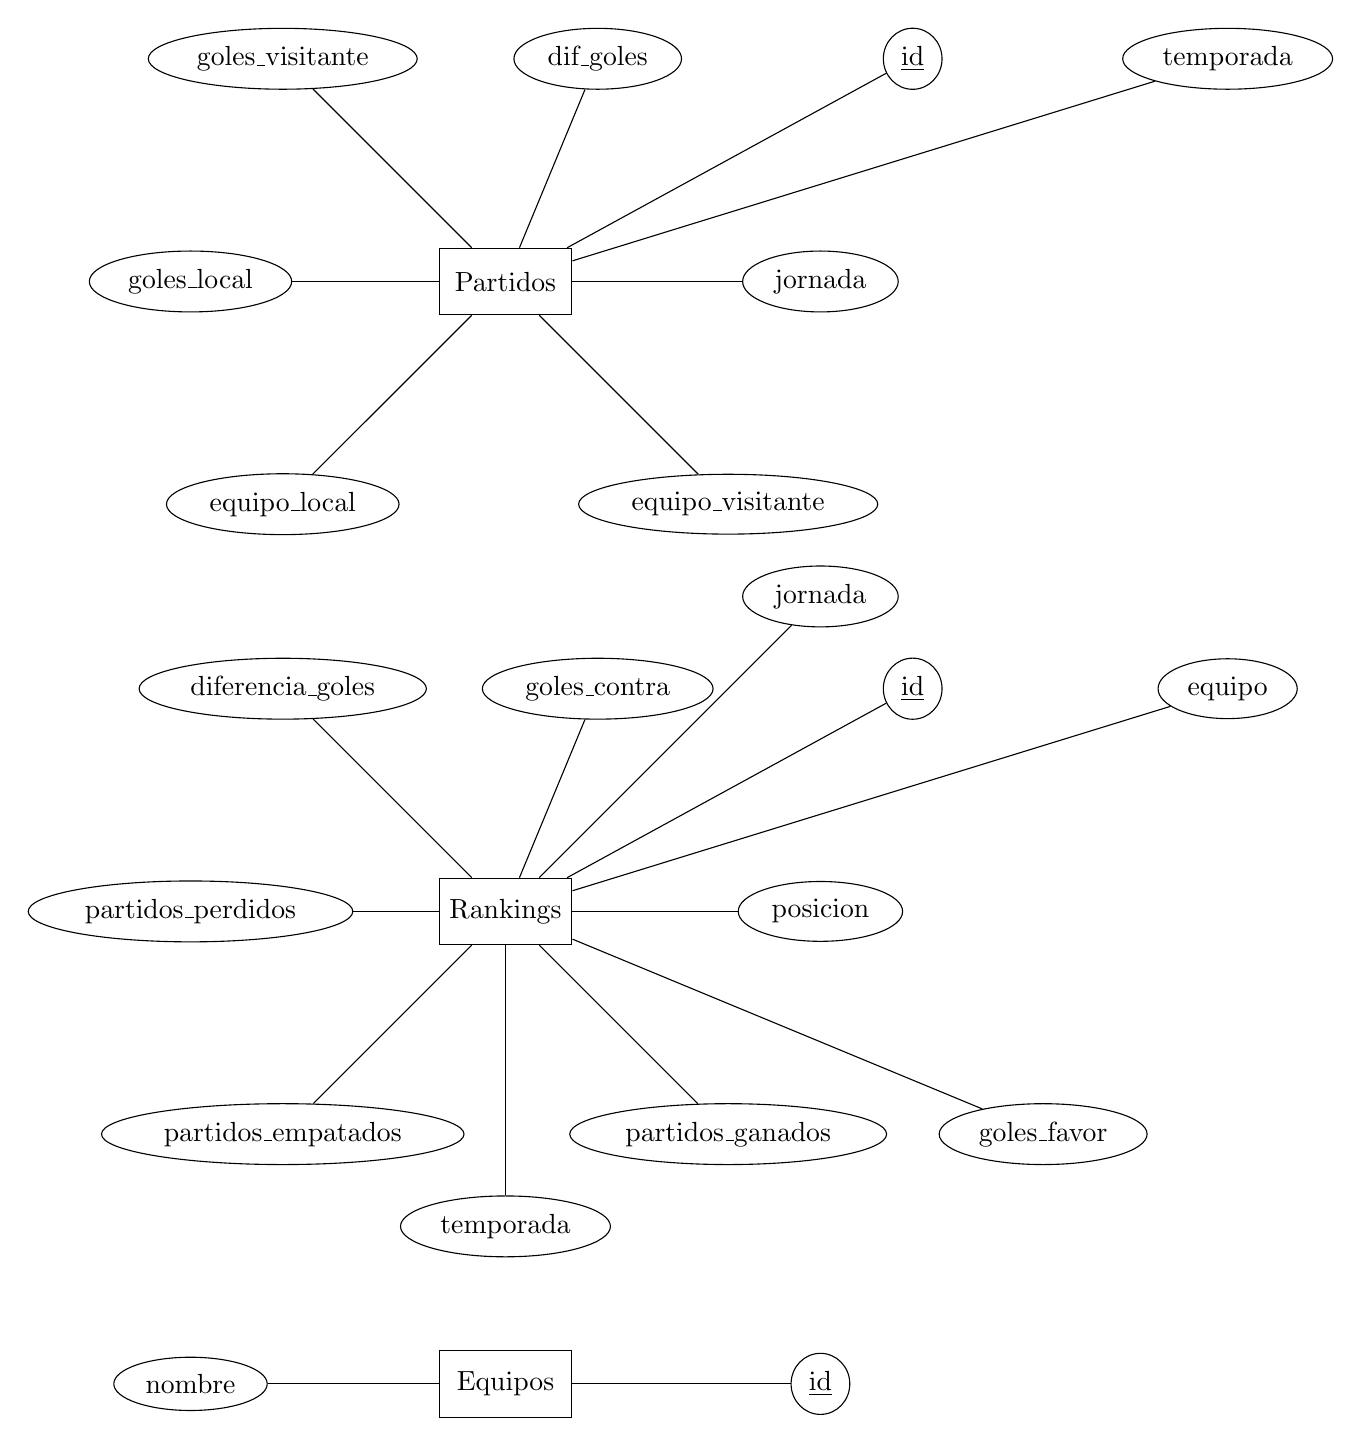
\begin{tikzpicture}[node distance=4cm]

% Partidos
\node [entity] (partidos) at (0,0) {Partidos};

\node [attribute] (goles_visitante) [above left of = partidos] { goles\_visitante } edge (partidos);

\node [attribute] (dif_goles) [right of = goles_visitante] { dif\_goles } edge (partidos);

\node [attribute] (p_id) [right of = dif_goles] { \key{id} } edge (partidos);

\node [attribute] (temporada) [right of = p_id] {temporada} edge (partidos);

\node [attribute] (jornada) [right of = partidos] { jornada } edge (partidos);

\node [attribute] (equipo_visitante) [below right of = partidos] { equipo\_visitante } edge (partidos);

\node [attribute] (equipo_local) [below left of = partidos] { equipo\_local } edge (partidos);

\node [attribute] (goles_local) [left of = partidos] { goles\_local } edge (partidos);

% Rankings
\node [entity] (rankings) at (0,-8) {Rankings};

\node [attribute] (diferencias_goles) [above left of = rankings] { diferencia\_goles } edge (rankings);

\node [attribute] (goles_contra_rankings) [right of = diferencias_goles] { goles\_contra } edge (rankings);

\node [attribute] (r_id) [right of = goles_contra_rankings] { \key{id} } edge (rankings);

\node [attribute] (equipo) [right of = r_id] { equipo } edge (rankings);

\node [attribute] (posicion) [right of = rankings] { posicion } edge (rankings);

\node [attribute] (partidos_ganados) [below right of = rankings] { partidos\_ganados } edge (rankings);

\node [attribute] (partidos_empatados) [below left of = rankings] { partidos\_empatados } edge (rankings);

\node [attribute] (partidos_perdidos) [left of = rankings] { partidos\_perdidos } edge (rankings);

\node [attribute] (goles_favor_rankings) [below right of = posicion] { goles\_favor } edge (rankings);

\node [attribute] (temporada_rankings) [below of = rankings] { temporada } edge (rankings);

\node [attribute] (jornada_rankings) [above of = posicion] { jornada } edge (rankings);

% Equipos

\node [entity] (equipos) at (0,-14) {Equipos};

\node [attribute] (nombre) [left of = equipos] {nombre} edge (equipos);

\node [attribute] (e_id) [right of = equipos] { \key{id} } edge (equipos);

\end{tikzpicture}}

\newcommand{\erapi}{
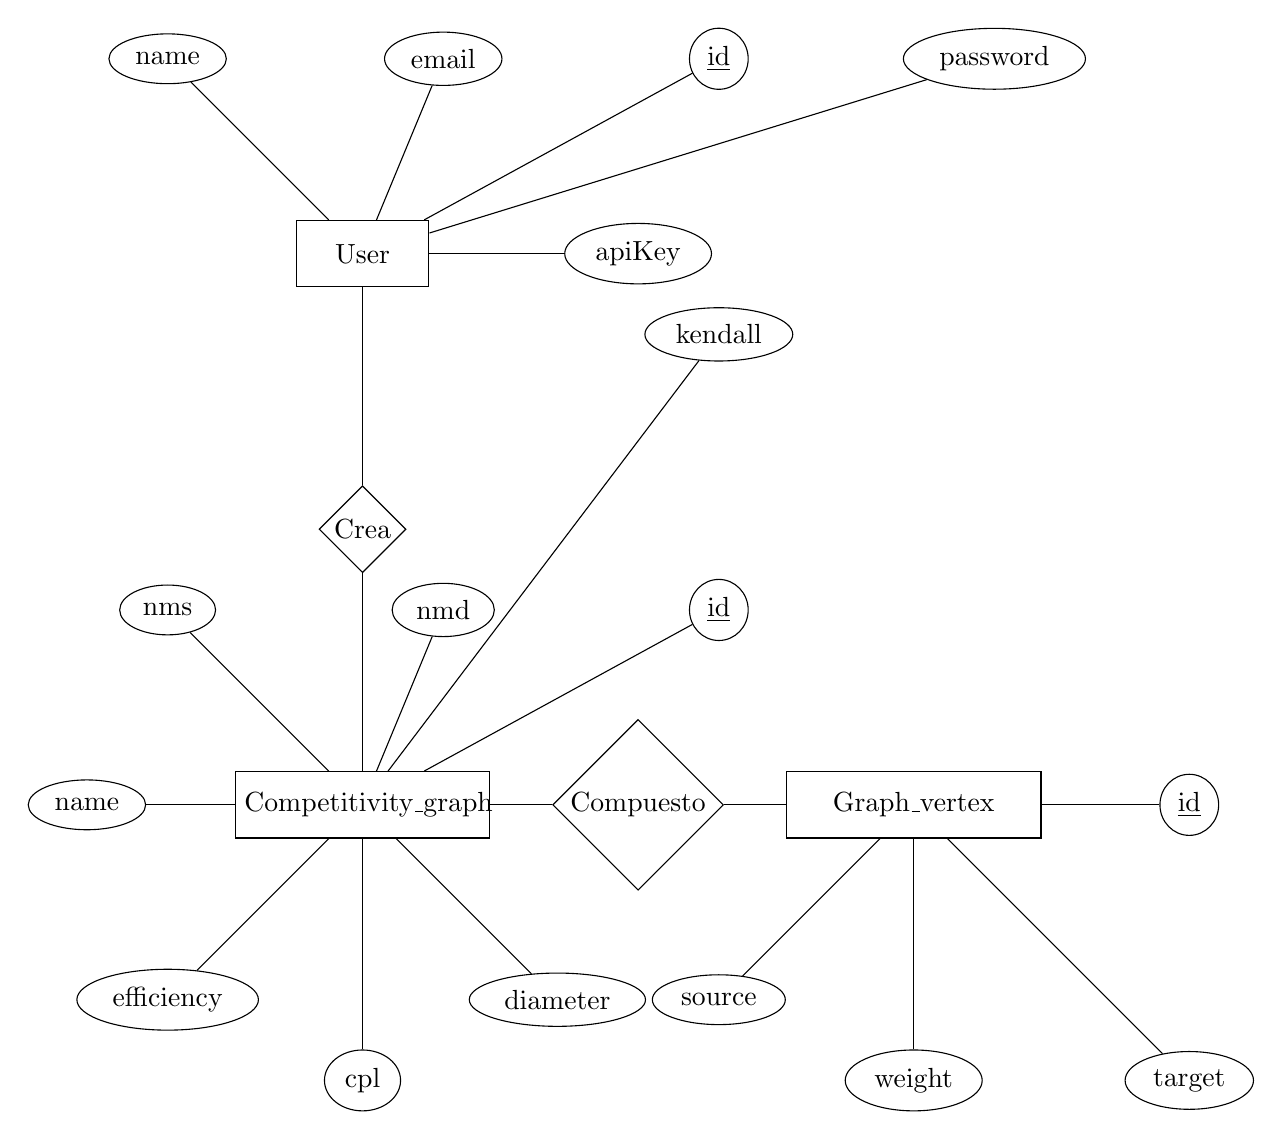
\begin{tikzpicture}[node distance=3.5cm]

% User
\node [entity] (user) at (0,0) {User};

\node [attribute] (name) [above left of = user] { name } edge (user);

\node [attribute] (email) [right of = name] { email } edge (user);

\node [attribute] (u_id) [right of = email] { \key{id} } edge (user);

\node [attribute] (password) [right of = u_id] {password} edge (user);

\node [attribute] (apiKey) [right of = user] { apiKey } edge (user);

\node [relationship] (crea) [below of = user] { Crea } edge (user);

% Competitivity graph
\node [entity] (competitivity) [below of = crea, text width=3cm, align=center] {Competitivity\_graph} edge (crea);

\node [attribute] (nms) [above left of = competitivity] { nms } edge (competitivity);

\node [attribute] (nmd) [right of = nms] { nmd } edge (competitivity);

\node [attribute] (c_id) [right of = nmd] { \key{id} } edge (competitivity);

\node [attribute] (kendall) [above of = c_id] {kendall} edge (competitivity);

\node [attribute] (cpl) [below of = competitivity] { cpl } edge (competitivity);

\node [attribute] (diameter) [below right of = competitivity] { diameter } edge (competitivity);

\node [attribute] (efficiency) [below left of = competitivity] { efficiency } edge (competitivity);

\node [attribute] (name) [left of = competitivity] {name} edge (competitivity);

\node [relationship] (compuesto) [right of = competitivity] {Compuesto} edge (competitivity);


% Graph vertex

\node [entity] (vertex) [right of = compuesto, text width=3cm, align=center] {Graph\_vertex} edge (compuesto);

\node [attribute] (source) [below left of = vertex] {source} edge (vertex);

\node [attribute] (v_id) [right of = vertex] { \key{id} } edge (vertex);


\node [attribute] (target) [below of = v_id] { target } edge (vertex);

\node [attribute] (weight) [below of = vertex] { weight } edge (vertex);

\end{tikzpicture}}